\label{chp:results}

After introducing the implementation of the \emph{ab initio} Green Kubo (aiGK) method in the previous chapter, we are now in position to present results for the set of potential thermal insulators identified in chapter~\ref{chp:anharmonicity}.

We first discuss the question of simulation time convergence for an initial set of materials in order to predict systems which can be computed with a simulation time of 30-60\,ps. This time was chosen as a compromise between the finite amount of available computational ressources and the desire to compute as many materials from the list of candidates as possible.
% 57 materials
%
In a second step, we compare the computed thermal conductivities at room temperature to experimental references for the subset of materials for which experiments are available to further verify the aiGK method beyond the two materials presented in the previous chapter.
% 22 materials 
%
In the last step, we present the computed thermal conductivities for the remaining materials,~i.\,e.,~those for which no experimental thermal conductivity was reported before, and discuss how they fit into the schema of predicting thermal insulators from anharmonicity estimates as discussed in Sec.\,\ref{sec:kappa_vs_sigmaA}. We eventually highlight the particularly interesting class of chalcopyrite compounds and try to answer some open questions from experimental and semi-empirical theoretical literature.

% \idea{compare to theoretical approaches, i.e., the Roekeghem perovskites}



\section{Convergence estimation}
We discuss simulation time convergence in the light of the \emph{effective simulation time} introduced in Sec.\,\ref{sec:implementation.convergece}. The key idea is to identify lower boundaries for the \emph{necessary} effective simulation time in a material in order to asses whether a time-converged thermal conductivity is possible to obtain within a simulation time of 30-60\,ps. For choosing these boundaries, we leverage the observed convergence behavior of seven materials,~i.\,e.,~MgO, NaF, KMgF$_3$, NaCl, NaBr, CuI, and NaI, each of them computed with 60\,ps simulation time. We thereby define four thresholds of minimal effective simulation time based on a material's anharmonicity $\sigmaA$, reflecting that phonons in harmonic materials like MgO have longer lifetimes than those in anharmonic materials. The criteria are displayed in Fig.\,\ref{fig:results.convergence}. In particular, we define the thresholds $\teff > 240$ for harmonic materials with $\sigmaA \leq 0.2$, $\teff > 120$ for materials with $0.2 < \sigmaA \leq 0.3$, $\teff > 60$ for materials with $0.3 < \sigmaA \leq 0.4$, and $\teff > 45$ for materials with $\sigmaA > 0.4$.

%The rational for this approach is that for individual materials, one would always compute several times longer trajectories to ensure that all relevant contributions are captured. In turn, several times less materials could be computed with a given amount of computational resources. Here, we leverage observations across different materials to circumvent this necessity for individual materials, thereby allowing to compute good estimates for thermal conductivity for dozens of them.
%
\begin{figure}
	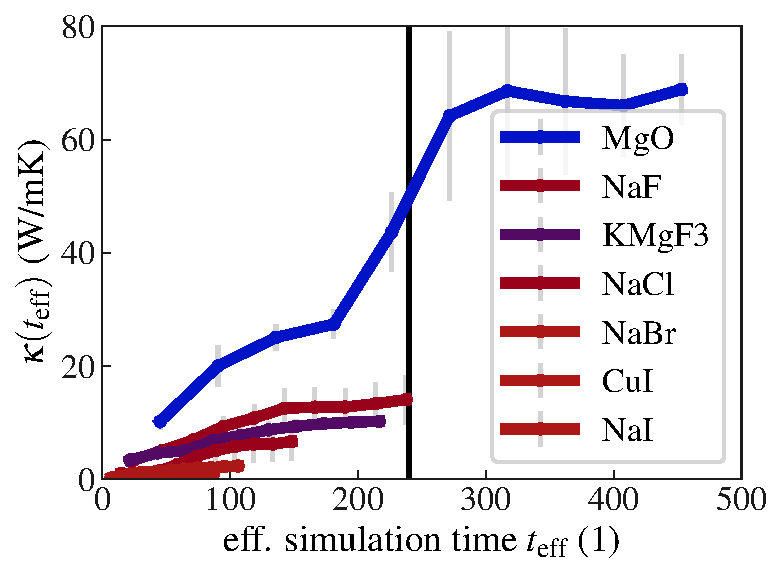
\includegraphics[width=.49\textwidth]{./data/plots/kappa_convergence/3.pdf}
	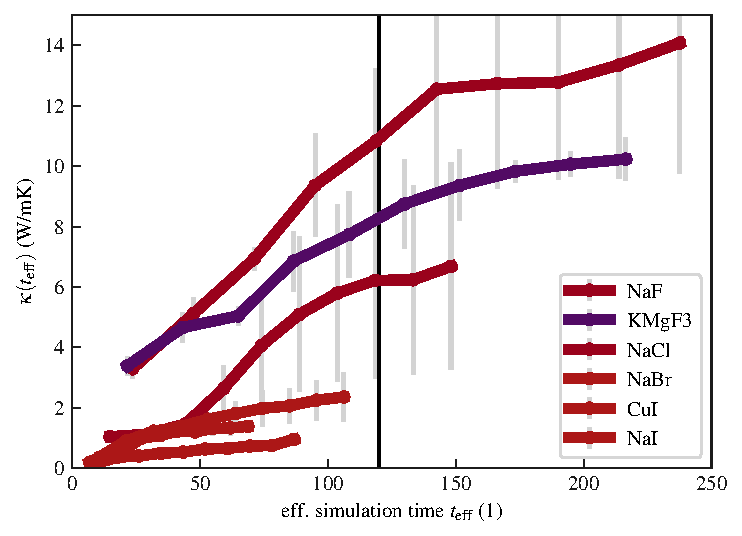
\includegraphics[width=.49\textwidth]{./data/plots/kappa_convergence/4.pdf}
	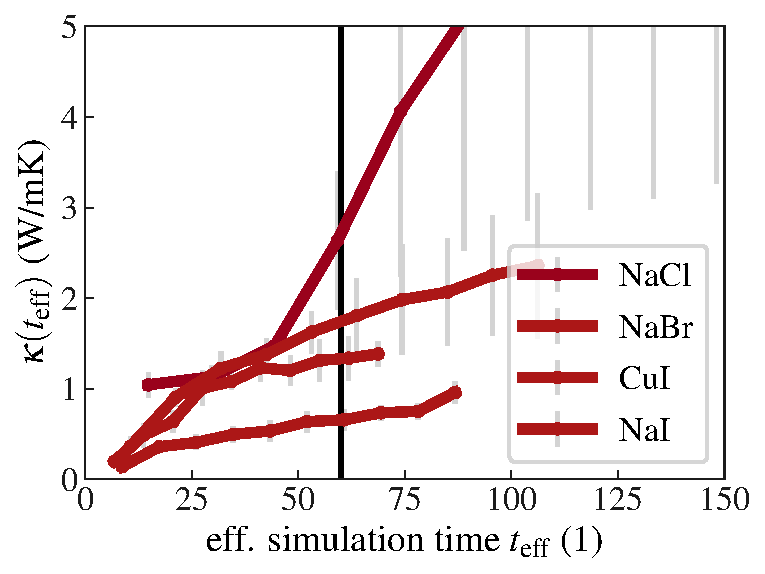
\includegraphics[width=.49\textwidth]{./data/plots/kappa_convergence/5.pdf}
	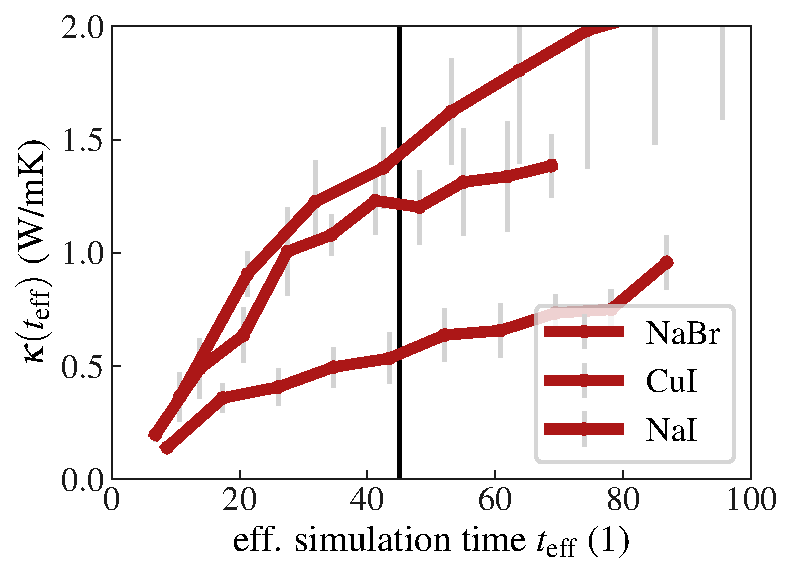
\includegraphics[width=.49\textwidth]{./data/plots/kappa_convergence/6.pdf}
	\caption{Illustration of minimal necessary effective simulation times. Upper left: $\teff = 240$ for harmonic materials with $\sigmaA \leq 0.2$. Upper right: $\teff = 120$ for materials with $0.2 < \sigmaA \leq 0.3$. Lower left: $\teff = 60$ for materials with $0.3 < \sigmaA \leq 0.4$. Lower right: $\teff = 45$ for materials with $\sigmaA > 0.4$.}
	\label{fig:results.convergence}
\end{figure}
%
We point out that at this stage, the given thresholds are meant as a \emph{necessary} condition for convergence, which ensures that a significant contribution to the cumulative thermal conductivity is included in the simulation. A statement about the \emph{sufficient} simulation time, however, can only made on the level of individual trajectories by means of longer simulation times. This verification should therefore be reserved for materials that show interesting properties after the \emph{necessary} simulation time.

Based on this estimation, we identify 57~materials out of the list of 112~candidates to compute thermal conductivity on, and discuss those in the following: First we compare thermal conductivities for 24 of these 57 materials to the experimental literature in order to benchmark the aiGK method, afterwards we present and discuss our findings for the remaining 33 materials without experimental reference.


\section{Comparison to experiment}
\label{sec:results.experiments}
In order to asses the validity of the aiGK method for the computation of thermal conductivity in anharmonic compounds, we compare results for 21 materials to the experimental literature. A detailed list including all considered experimental references is given in Tab.\,\ref{tab:kappa.exp} in appendix~\ref{sec:app.experiments}. The difficulties when comparing to experimental references have been discussed in detail for periclase MgO in Sec.\,\ref{sec:mgo.experiments}. In principle, these carry over to all other compounds, however, for most materials, the body of literature is much smaller compared to MgO. The list of experiments also includes measurements on polycrystalline samples. While thermal conductivity should be reduced in polycrystalline samples compared to single crystals because of boundary scattering, experimental studies have shown that the effect is minor in sufficiently dense polycrystalline samples, especially in low thermal conductivity materials which are less sensitive to boundary scattering due to their intrinsically low phonon mean free paths~\cite{Charvat.1957}. In the course of our literature review we have generally found differences of 0-20\,\% between measurements on single- and polycrystalline samples, which supports this finding. Nevertheless, additional care must be taken when evaluating literature on polycrystalline samples: Experiments aiming at measuring other properties besides thermal conductivity, in particular the thermoelectric figure of merit $zT$, typically do not attempt to reproduce the bulk thermal conductivity, and use less dense samples, which is beneficial for reducing thermal conductivity and thereby increasing the figure of merit. The resulting thermal conductivity will then be determined mostly by the details of the sample processing, 
%\mscomment{this is true for all experimental data}
%\FK{I disagree, actual bulk properties are somewhat robust against minor manufacturing differences. Clarify: I mean here that sampling process \emph{significanlty} determines the properties beyond single-digit deviations.}
and a comparison to bulk thermal conductivity is not meaningful. However, some experiments specifically aim at reproducing polycrystalline samples of near-bulk density in order to assess the bulk thermal conductivity of a material. Only experiments on polycrystalline samples of this type are considered in this work.

A comparison of thermal conductivities computed via the aiGK method as introduced in the previous chapter and the experimental literature is shown in Fig.\,\ref{fig:kappa_exp}.
%
\begin{figure}
	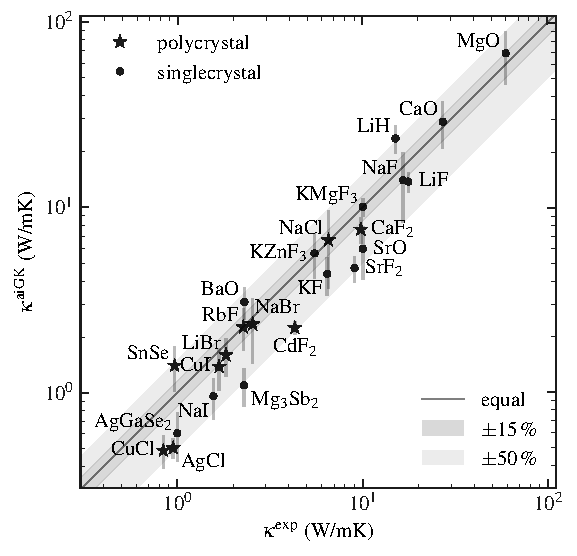
\includegraphics[width=\textwidth]{./data/plots/kappa_vs_exp_trusted/kappa_vs_exp_corrected_annotated.pdf}
	\caption{Comparison to experiment. Bullets($\bullet$): Single crystal. Stars ($\star$): Contains data from polycrystalline experiment. Error bar in y-direction: Statistical uncertainty for $\kappa^{\rm aiGK}$ from standard error over individual trajectories. Diagonal line: Agreement with experiment or mean of experiments if multiple available. Dark grey region: Agreement between mean experiment and mean computation with $\pm 15\,\%$ deviation. Light grey region: Agreement between mean experiment and mean computation with $\pm 50\,\%$ deviation.}
	\label{fig:kappa_exp}
\end{figure}
%
Overall, we find very good agreement in the 24 considered materials, with 10 out of 24 being within experimental accuracy of $\pm 15\,\%$, and all other within an extended %experimental 
accuracy which we choose as $\pm 50\,\%$ within the average experimental reference, reflecting the high degree of variation in experimental values for materials where a significant amount of references is available, see our discussion for MgO in Sec.\,\ref{sec:mgo.experiments} and the discussion in Ref.\,\cite{Wei.2016}. A list of the computed values including simulation times and corresponding effective simulation time is given in Tab.\,\ref{tab:kappa.w/exp} below.

\begin{marginfigure}
	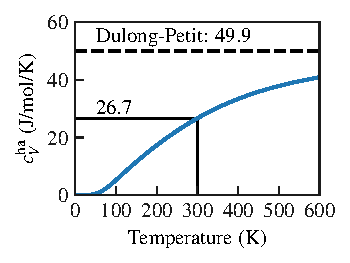
\includegraphics[width=\textwidth]{./data/plots/heat_capacity/225.LiH/thermal_properties.pdf}
	\caption{Harmonic heat capacity per formula unit $c_V^{\rm ha}$ for LiH compared to the classical Dulong-Petit value.}
	\label{fig:LiH.cv}
\end{marginfigure}
%
The strongest deviation from experiment is seen for LiH, which is computed as $\kappa^{\rm aiGK} = 23.6 \pm 4.0$\,W/mK, where the available experimental value is $\kappa^{\rm exp} = 14.7$\,W/mK~\cite{Slack.1973}. However, both lithium and especially hydrogen are light elements, so that LiH is not fully classical at room temperature, as can be estimated by comparing the harmonic heat capacity of LiH at 300\,K to the classical Dulong-Petit value in Fig.\,\ref{fig:LiH.cv}~\cite{Dove}. The harmonic heat capacity for LiH is only at about 50\,\% of the classically expected value of $6 R = 49.9$\,J/mol/K for solids with two atoms in the unitcell. This value can only be taken as an upper boundary to the deviation in thermal tranpsort properties expected from the lack of nuclear quantum effects, since low-frequency phonon modes already behave more classical at the given temperature~\cite{Volz.2020,Volz.2020b}. A significant overestimation by the classical Green Kubo method can nevertheless be expected in this material.\footnote{We evaluated several schemes to quantitatively correct for nuclear quantum effects~\cite{Wang.1990,Maiti.1997}, however, the literature seems to agree that this is an open problem for thermal conductivity in bulk solids, see in particular discussions in Ref.~\cite{Turney.2009,Puligheddu.2019}.}
%\mscomment{There have been efforts to estimate ZP/NQE effects, why wouldn't this improve the estimate?}
%\FK{The approaches I found were dealing with elemental solids. Li is 7 times heavier than H, so uniform scaling e.g. by correcting the temperature based on the heat capacity would, from my point of view, do more harm than good. It would give a correction into the right direction for the not-so-right reasons.}
Interestingly, the aiGK value agrees very well with another computational study by Lindsay, who found a value of $\kappa = 23.00$\,W/mK using third-order Boltzmann transport~\cite{Lindsay.2016}.\footnote{Lindsay used an LDA exchange-correlation functional, which thermal conductivity can deviate $\pm 20\,\%$ from the PBEsol functional used in this work~\cite{Carbogno.2016}. However, the disagreement with experiment is still significantly larger then the potential inaccuracy stemming from the xc functional.} In that approach, the quantum nature of nuclei should be better captured than in the aiGK method, and Lindsay ascribes the deviation from experiment to higher-order phonon-phonon interactions neglected in their approach. This discussion is in line with the more phenomenological discussion proposed by Slack in Ref.\,\cite{Slack.1973}, where he points out the strong anharmonicity in LiH that manifests in the change of phonon frequencies as measured by the Gr\"uneisen parameter. Indeed, in our study we find a value of $\sigmaA = 0.30$ for the strength of anharmonicity in LiH, which can be expected to be even larger when nuclear quantum effects are considered.\footnote{Nuclear quantum effects increase the anharmonic strength of LiH at room temperature by about 20\,\%~\cite{hengst1}.} We therefore suggest LiH as an interesting yet simple candidate for studying the interplay of strong anharmoncity and nuclear quantum effects in bulk solids in future work.
%
\begin{marginfigure}
	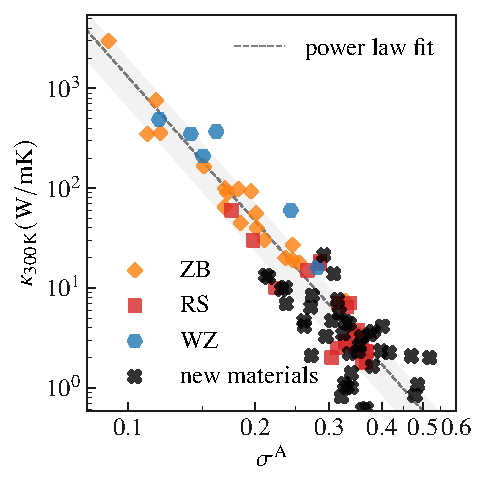
\includegraphics[width=\textwidth]{./data/plots/anharmonicity/9_kappa/incl_computations/sigma_vs_kappa_annot_comp_margin.pdf}
	\caption{
%	\mscomment{too crowded}
	Thermal conductivity at room temperature vs. anharmonicity measure. ZB: zincblende, RS: rock salt, WZ: wurtzite, cf. Fig.\,\ref{fig:anh.kappa}.}
	\label{fig:kappa_sigma_exp_comp}
\end{marginfigure}
%
\begin{marginfigure}
	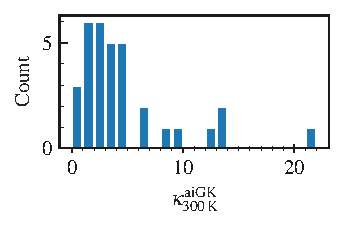
\includegraphics[width=\textwidth]{./data/plots/kappa_histogram/histogram.pdf}
	\caption{Summary of the range of thermal conductivities for materials without experimental reference found in this study.}
	\label{fig:kappa_wo_exp_hist}
\end{marginfigure}

Another noteworthy material in the list is SnSe: We predict the thermal conductivity of SnSe to be $1.40 \pm 0.38$\,W/mK, which is on the upper limit of the experimental references and agrees reasonably with the measurements by Wei and coworkers on near-bulk-density polycrystalline samples yielding a value of $\kappa = 1.3$\,W/mK~\cite{Wei.2016}.
However, this value is twice as big as the ultralow thermal conductivity of $0.6$\,W/mK reported in the seminal work on record-high thermoelectric figure of merit in Snse by Zhao and coworkers~\cite{Zhao.2014}. Our findings support the critique of Wei and coworkers that the SnSe crystals studied by Zhao and coworkers contained a non-negligible amount of defects and were heavily modified structurally, as reflected by an approximately 10\,\% lower density of the studied samples compared to theoretical bulk limit and measurements reported by other groups~\cite{Wei.2016}.



\section{New materials and relation to anharmonicity}
\label{sec:results.new}
After validating the aiGK method against experimental literature, we present results for 33~materials \emph{without} experimental reference. We display these values in the context of the $\kappa$ vs. $\sigmaA$ plot introduced in Fig.\,\ref{fig:anh.kappa}, where we identified a power-law relation of experimental thermal conductivities with the anharmonicity measure $\sigmaA$ for simple elementary and binary materials. We show the data again in Fig.\,\ref{fig:kappa_sigma_exp_comp}, but this time including the additional, non-experimentally measured materials computed in this work.
%
It is apparent that the correlation between thermal conductivity $\kappa$ and $\sigmaA$ carries over from the simple materials to the more complex binary and ternary compound classes studied in this work, since the power-law fit in Fig.\,\ref{fig:kappa_sigma_exp_comp} is still performed with respect to the experimental values initially presented in Fig.\,\ref{fig:anh.kappa}. While the overall trend of decreasing thermal conductivity with increasing anharmonicity is clearly preserved, the spread of $\kappa$ values for materials with similar $\sigmaA$ or vice versa increases, which is expected due to the increased structural and chemical complexity of the studied materials.

Focusing on the new materials, we show a zoomed-in part of the $\kappa-\sigmaA$ plane in Fig.\,\ref{fig:kappa_sigma}, with only computational data, highlighting the materials where no experimental reference is available.
%
\begin{figure*}
	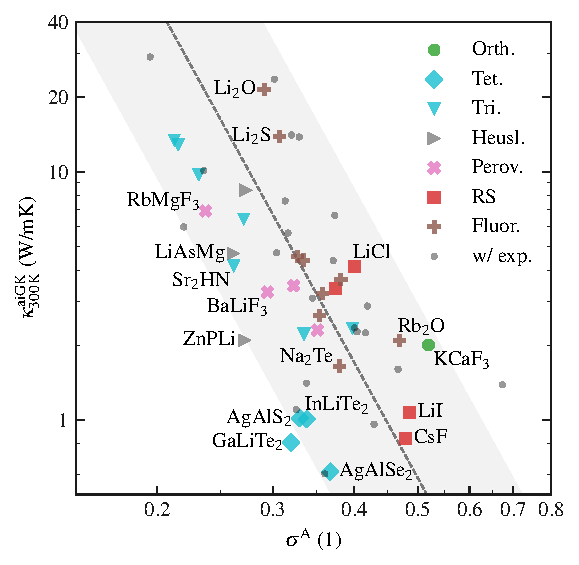
\includegraphics[width=.49\textwidth]{./data/plots/kappa_vs_sigma_trusted/kappa_vs_sigma_trusted.pdf}
	\hfill
	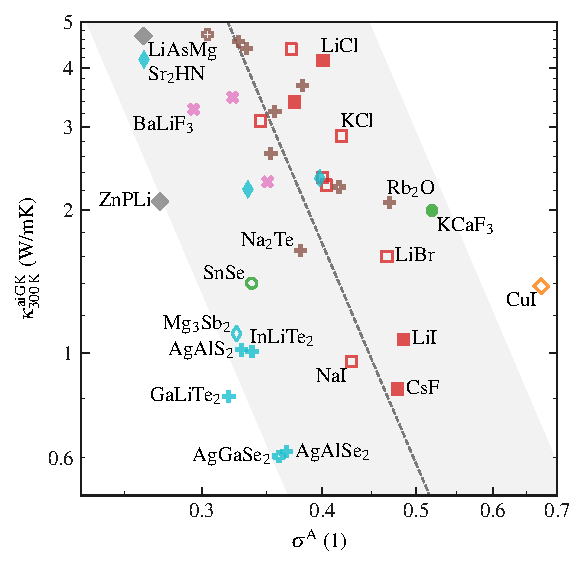
\includegraphics[width=.49\textwidth]{./data/plots/kappa_vs_sigma_trusted/kappa_vs_sigma_trusted_experiment_zoom.pdf}
	\caption{
	Thermal conductivity at room temperature computed via \emph{ab initio} Green Kubo (aiGK) vs. anharmonicity measure. Filled symbols denote materials without experimental reference. Left: Overview of studied materials without experimental reference. Materials with experimental reference are included as small dots for reference. Right: Zoom into the region $\kappa \leq 5$\,W/mK. Open symbols represent materials where experimental reference is available. The dashed line and shaded area are the same as in Fig.\,\ref{fig:kappa_sigma_exp_comp},~i.\,e.,~they represent a power-law fit to experimental thermal conductivities and a $\pm 50\,\%$ margin.}
	\label{fig:kappa_sigma}
\end{figure*}
%
In particular, we find 28 new materials with a computed bulk thermal conductivity of $\kappa^{\rm aiGK} < 10\,{\rm W/mK}$, 24 of which show $\kappa^{\rm aiGK} < 5\,{\rm W/mK}$, and 8 with $\kappa^{\rm aiGK} \leq 2\,{\rm W/mK}$,~i.\,e.,~comparable to the bulk thermal conductivity of existing and candidate thermoelectric materials such as Bi$_2$Te$_3$ and Bi$_2$Se$_3$ (1.3\,W/mK~\cite{Goldsmid.1956,Satterthwaite.1957}), PbTe (2.0\,W/mK~\cite{Elsharkawy.1983}), SnSe (1\,W/mK~\cite{Zhao.2014,Wei.2016,Sassi.2014}), M$_2$Sb$_3$ (2.3\,W/mK~\cite{Ahmadpour.2007,Pan.2020}), or GeTe (2.5\,W/mK~\cite{Perumal.2015}). A full list of all values is given in Tab.\,\ref{tab:kappa.noexp}, and a histogram of the values is shown in Fig.\,\ref{fig:kappa_wo_exp_hist}. The materials of very low thermal conductivity comprise simple binary, cubic materials such as the rock salt structures CsF ($\kappa^{\rm aiGK} = 0.84$) and LiI ($\kappa^{\rm aiGK} = 1.07$), or the fluorite structure Na$_2$Te ($\kappa^{\rm aiGK} = 1.64$), but also more complex structures such as the strongly anharmonic perovskites KCdF$_3$ ($\kappa^{\rm aiGK} = 1.67$) and KCaF$_3$ ($\kappa^{\rm aiGK} = 2.00$).


\subsection{Chalcopyrite systems}
\label{sec:chalcopyrites}
Particularly noteworthy is a class of ternary materials, so-called \emph{chalcopyrites}, a tetragonal crystal class closely related to the zincblende structure~\cite{Wasim.1979}. These crystals have been studied in the past primarily because of their non-linear optical properties~\cite{Ho.2014}, but also thermal transport properties have been studied~\cite{Spitzer.1970,Wasim.1979,Garbato.1979}, mainly because thermal transport can limit the optical efficiency in these devices~\cite{Beasley.1994}. However, experimental references for this class of materials are scarce, and do not agree well~\cite{Beasley.1994}. 
%
\begin{table}[ht]
  \centering
  \fontfamily{ppl}\selectfont
  \begin{tabulary}{\textwidth}{LC}
    \toprule
    Reference & Thermal conductivity at 300\,K (W/mK) \\
    \midrule
    Berger 1966 (experiment)~\cite{berger1969}   & $2.7$          \\
    Beasley 1995 (experiment)~\cite{Beasley.1994} & $1.1$          \\
    This work (theory)                           & $0.6 \pm 0.2$  \\
    \bottomrule
    \vspace{.5em}
  \end{tabulary}
  \caption{Overview of experimental references for AgGaSe$_2$.}
  \label{tab:exp.aggase2}
\end{table}
%
Picking AgGaSe$_2$ as an example, there are two distinct measurements available as summarized in Tab.\,\ref{tab:exp.aggase2}, ranging from $1.1-2.7$\,W/mK~\cite{Beasley.1994,berger1969}. These values are complemented by calculated values based on semi-empirical models, ranging from $4.8-9.0$\,W/mK~\cite{Wasim.1979,Rincon.1995}. Our computed thermal conductivities are collected in Tab.\,\ref{tab:exp.chalcopyrites}.
%
\begin{table}[ht]
  \centering
  \fontfamily{ppl}\selectfont
  \begin{tabularx}{\textwidth}{lXcXc}
    \toprule
    Material & & $\kappa^{\rm aiGK}$ (W/mK) & & $\sigmaA$ \\
    \midrule
	  AgAlS$_2$   & & $1.01 \pm 0.20$ & & 0.33 \\
          AgAlSe$_2$  & & $0.62 \pm 0.16$ & & 0.37 \\
          AgGaSe$_2$  & & $0.61 \pm 0.18$ & & 0.35 \\
          GaLiTe$_2$  & & $0.81 \pm 0.15$ & & 0.31 \\
          InLiTe$_2$  & & $1.01 \pm 0.26$ & & 0.33 \\
    \bottomrule
    \vspace{.5em}
  \end{tabularx}
  \caption{Overview of computed thermal conductivities for chalcopyrite materials.}
  \label{tab:exp.chalcopyrites}
\end{table}

Besides AgGaSe$_2$, there is experimental reference for the chemically closely related material, AgGaS$_2$, with a measured thermal conductivity of 1.4\,W/mK~\cite{Beasley.1994}.
%\footnote{While we included AgGaS$_2$ in our dataset, we needed to discard the material because of aiMD convergence problems. 
%\mscomment{what kind of problems?}
%However, we like to mention this material in the context of this study as potentially interesting material for future investigations.} 
While our computational data might underestimate the thermal conductivity in these compounds slightly\footnote{Please keep in mind, that the absolute errors are only of the order of 0.5-1\,W/mK.}, we nevertheless see a clear indiciation of very low intrinsic thermal conductivity in AgGaSe$_2$, and the chemically closely related compounds AgAlS$_2$ and AgAlSe$_2$. At least regarding their thermal transport properties, they are therefore comparable or even superior to the existing thermoelectric materials listed in the previous section, while being free of heavy metals such as Pb or Bi.
The class of chalcopyrite materials has recently been investigated in a high-throughput study conducted by Plata and coworkers~\cite{Plata.2021pre}. Their findings are overall in line with ours, supporting the finding that the class of chalcopyrite materials may comprise several promising thermal insulators.
 % Mg$_3$Sb$_2$~\cite{kajikawa2003,Condron.2006,Zhang.2009,Zhang.2018,Pan.2020,Ding.2021}.
%\todo{$\kappa_{\rm MgSb}^{\rm aiGK} = 1.10 \pm 0.26$}

To qualitatively elucidate the nuclear dynamics of the chalcopyrite systems, we present phonon spectral functions obtained from a temperature dependent model Hamiltonian for the nuclear system up to third-order displacements to estimate phonon-phonon interactions in Fig.\,\ref{fig:sqe_all}~\cite{Hellman.2013,Hellman.2013b,Squires}.
%
\begin{figure}
	\centering
	AgGaSe2$_2$ \hspace{3.7cm} AgAlSe$_2$\\
	% \includegraphics[width=0.49\textwidth]{./data/plots/spectral_functions/122.04.AgGaS2.12.png}
	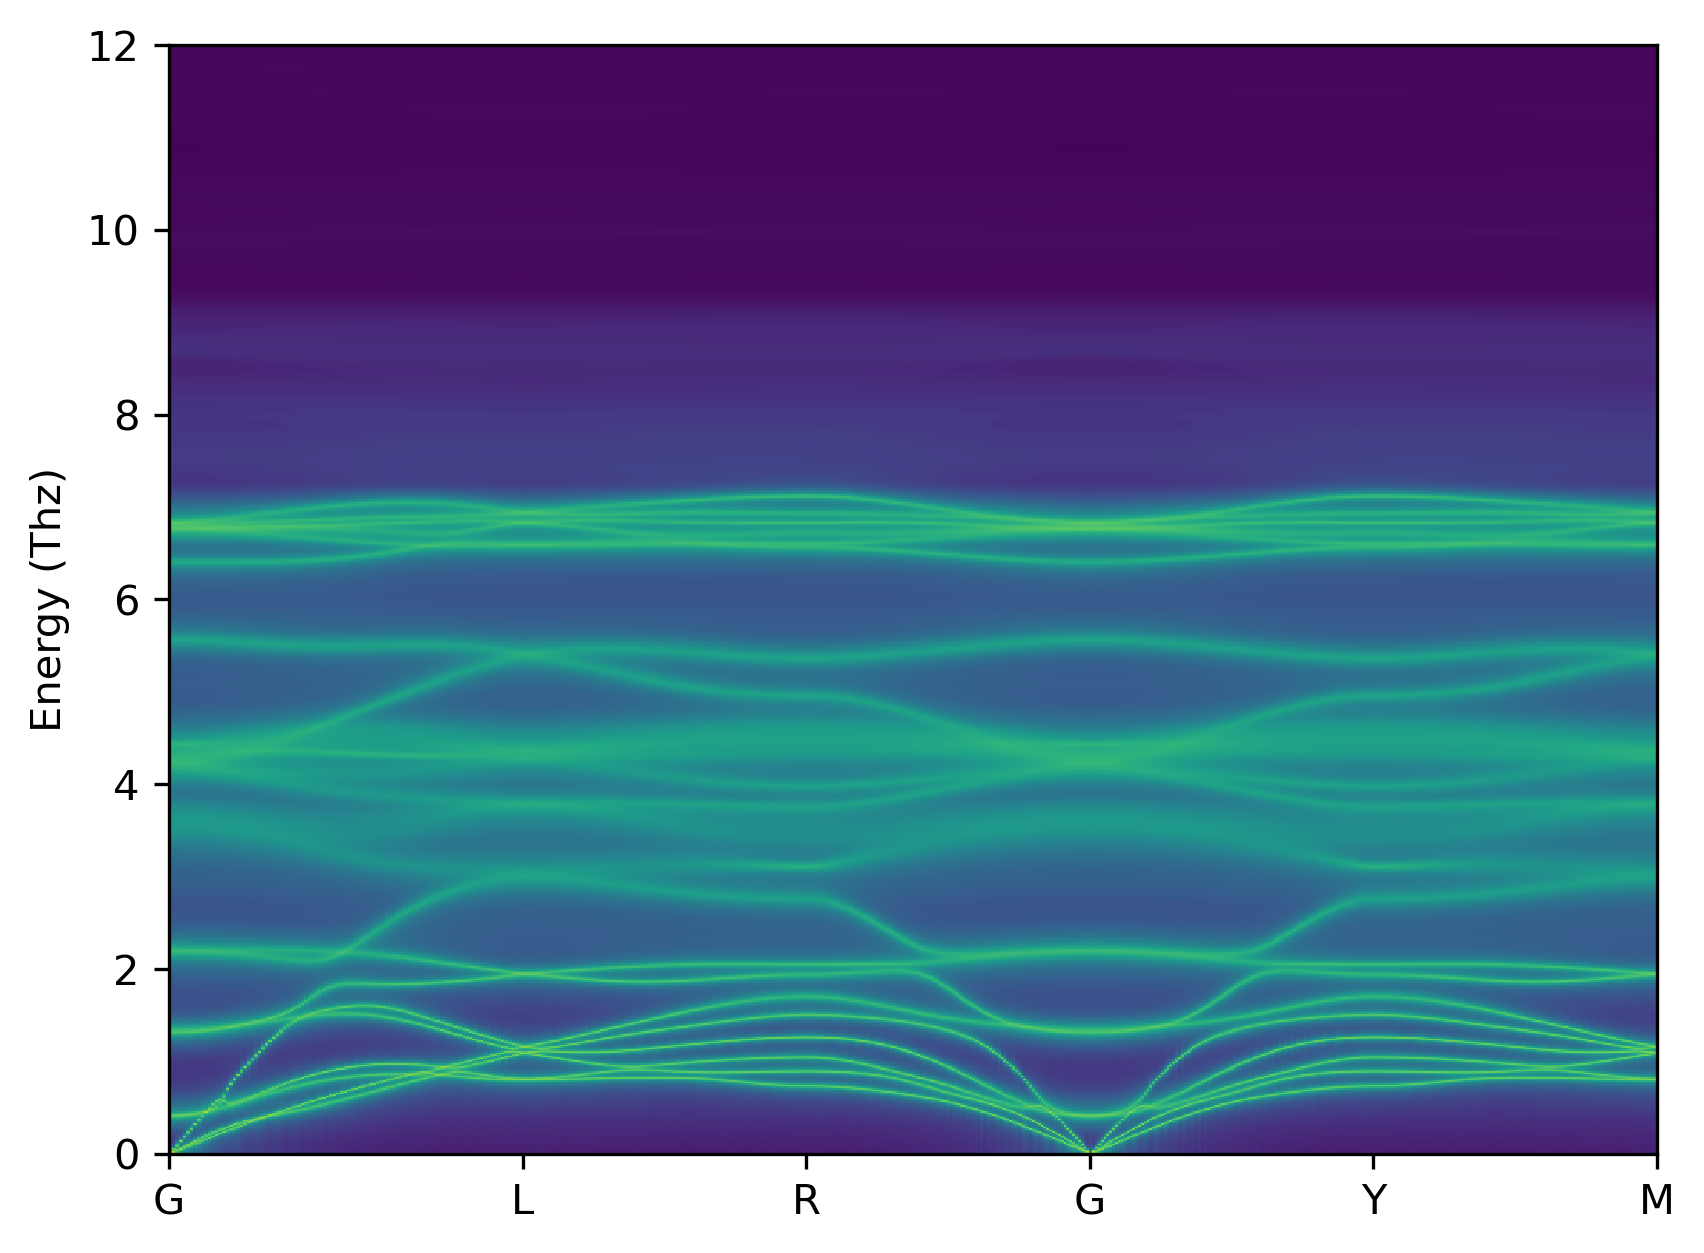
\includegraphics[width=0.49\textwidth]{./data/plots/spectral_functions/122.04.AgGaSe2.12.png}
	%	AgAlS$_2$ \hspace{3.7cm} AgAlSe$_2$\\
	%\includegraphics[width=0.49\textwidth]{./data/plots/spectral_functions/122.04.AgAlS2.15.png}
	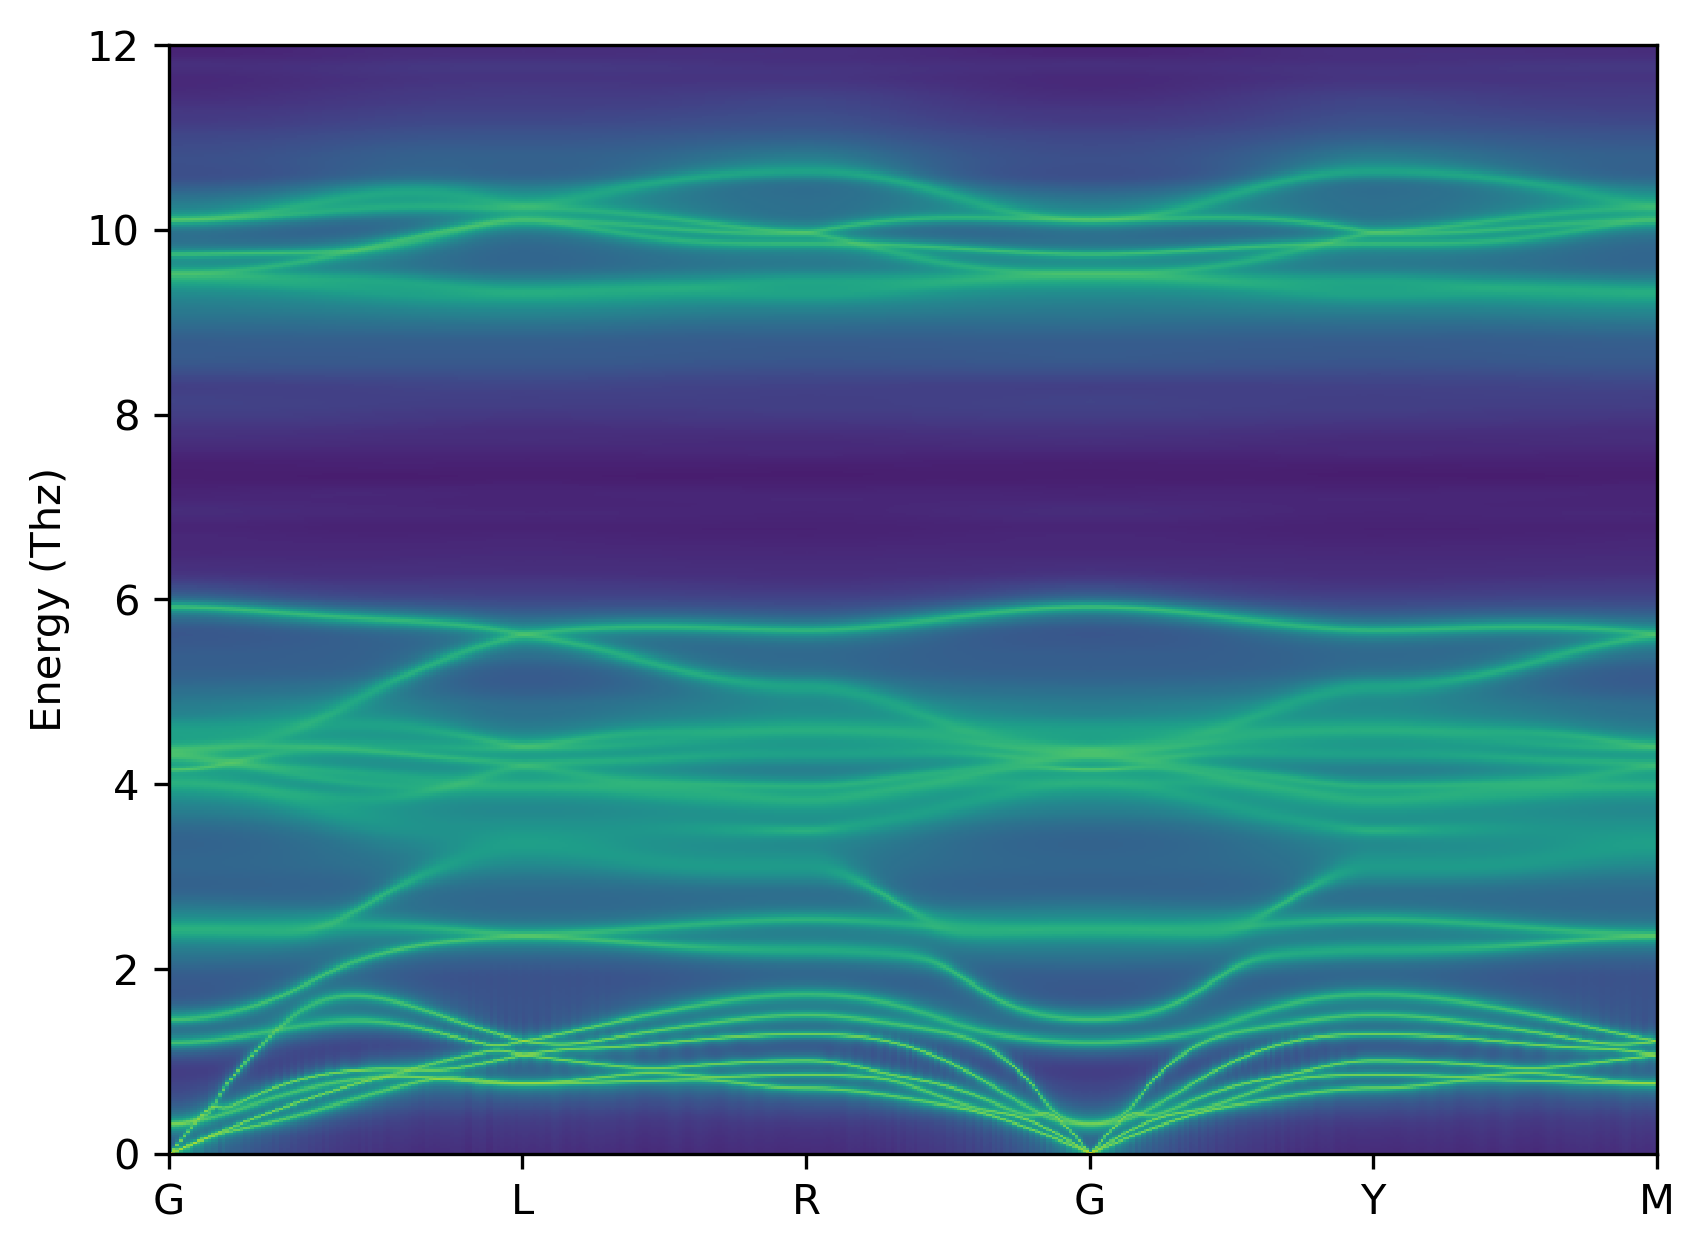
\includegraphics[width=0.49\textwidth]{./data/plots/spectral_functions/122.04.AgAlSe2.12.png}
	\\
	GaLiTe$_2$ \hspace{3.7cm} InLiTe$_2$\\
	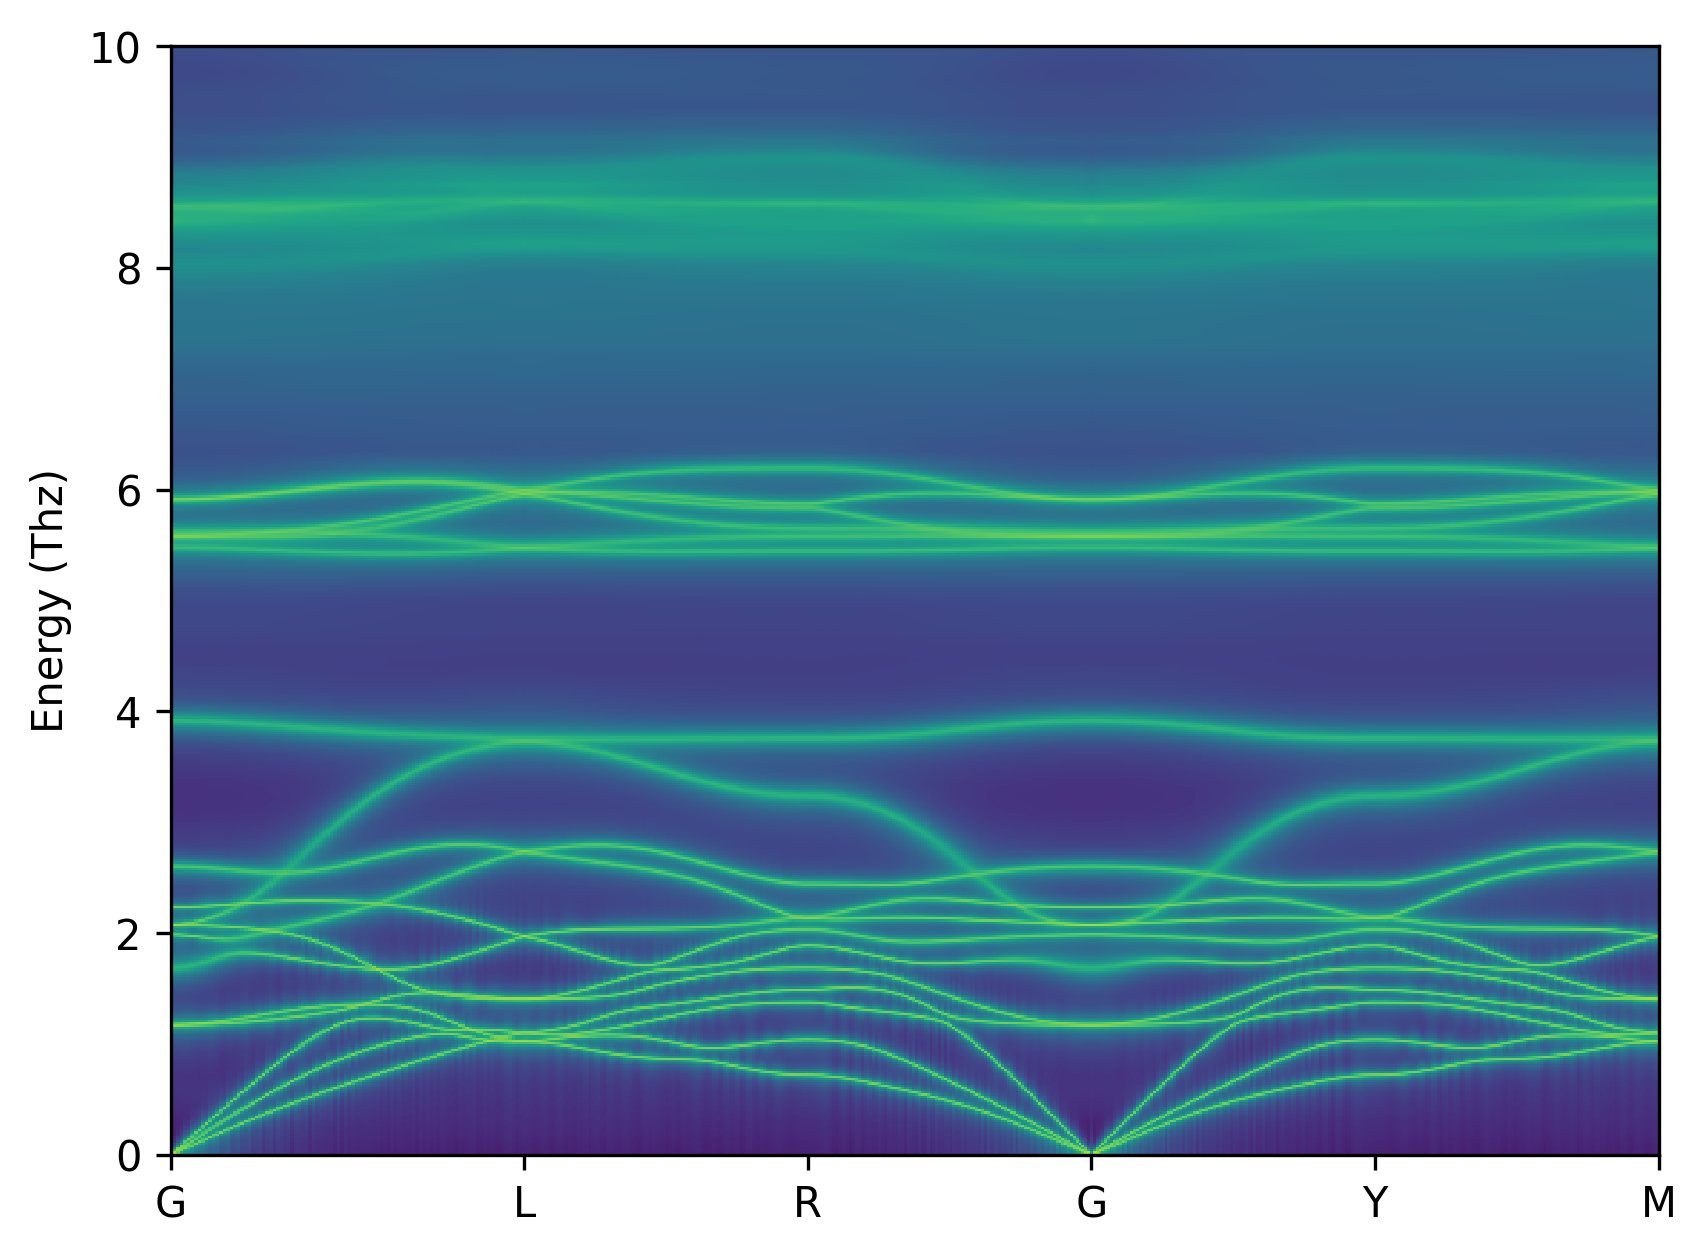
\includegraphics[width=0.49\textwidth]{./data/plots/spectral_functions/122.04.GaLiTe2.png}
	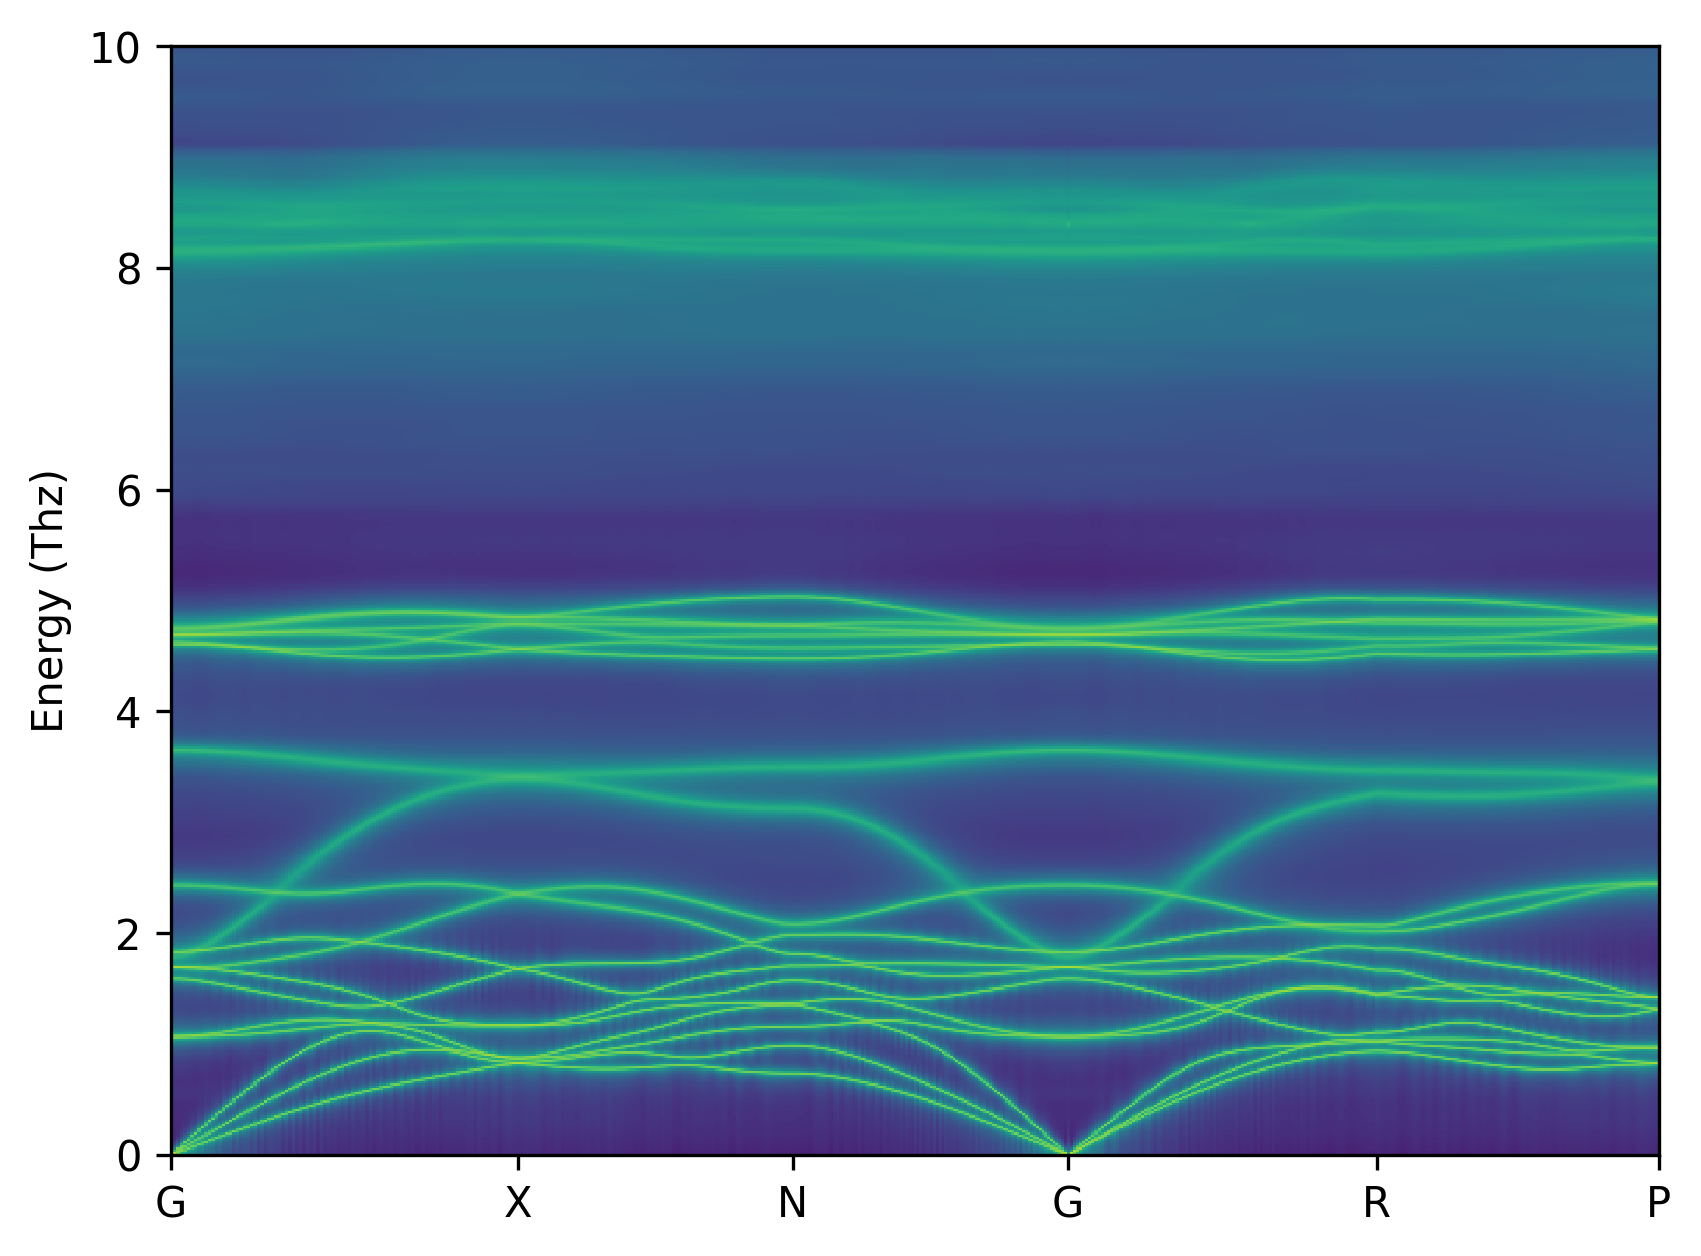
\includegraphics[width=0.49\textwidth]{./data/plots/spectral_functions/122.04.InLiTe2.png}
	\caption{Spectral functions for the chalcopyrite materials, AgGaSe$_2$, AgAlSe$_2$, GaLiTe$_2$, and InLiTe$_2$.}
	\label{fig:sqe_all}
\end{figure}
%
The common feature of these dispersions are the very flat acoustic branches which vary less than 1\,THz across the entire Brillouin zone, and a multitude of flat, nearly degenerate optical branches showing very litte to no dispersion. From a phonon-theory point of view, non-dispersive branches correspond to localized atomic motion in the system and therefore carry little heat beyond the Einstein-like diffusion of thermal energy from atom to atom, which is the dominant heat transport mechanism in structurally disordered systems like glasses~\cite{Simoncelli.2019}. Furthermore, in particular the optical branches are substantially broadened, which corresponds to strong anharmonic coupling in these systems, reducing their thermal conductivity.
%
\begin{table}[ht]
  \centering
  \fontfamily{ppl}\selectfont
\begin{tabularx}{\linewidth}{rXXXrr}
\toprule
Space group  &    material & $\kappa^{\rm aiGK}$ (W/mK) & $\sigmaA$  & $t_{\rm sim}$ (ps)  & $t_{\rm eff}$ (1) \\
\midrule
         122 & AgAlSe$_2$ &             0.62 &       0.37 &         60 &      90.50 \\
         122 & GaLiTe$_2$ &             0.81 &       0.32 &         60 &     195.78 \\
         225 &        CsF &             0.84 &       0.48 &         30 &      51.68 \\
         122 & InLiTe$_2$ &             1.01 &       0.34 &         60 &     192.73 \\
         122 &  AgAlS$_2$ &             1.01 &       0.33 &         60 &     125.88 \\
         225 &        LiI &             1.07 &       0.49 &         30 &      92.67 \\
         225 &   Na$_2$Te &             1.64 &       0.38 &         30 &      62.88 \\
          62 &   KCdF$_3$ &             1.67 & 0.53$^\dagger$ &     30 &      57.29 \\
          62 &   KCaF$_3$ &             2.00 &       0.52 &         30 &      65.03 \\
         225 &    Rb$_2$O &             2.08 &       0.47 &         30 &      51.66 \\
         216 &      ZnPLi &             2.09 &       0.27 &         30 &     148.55 \\
         166 & InNaSe$_2$ &             2.22 &       0.34 &         30 &      61.30 \\
         221 &  CsCdF$_3$ &             2.30 &       0.35 &         30 &      76.13 \\
         166 & InLiSe$_2$ &             2.34 &       0.40 &         30 &      88.77 \\
         225 &   Na$_2$Se &             2.63 &       0.35 &         30 &      70.78 \\
         225 &   Li$_2$Te &             3.24 &       0.36 &         30 &     163.92 \\
         221 &  BaLiF$_3$ &             3.27 &       0.29 &         60 &     238.35 \\
         225 &         KH &             3.39 &       0.37 &         30 &     324.72 \\
         221 &  RbZnF$_3$ &             3.47 &       0.32 &         60 &     201.23 \\
         225 &     K$_2$O &             3.67 &       0.38 &         30 &      65.37 \\
         225 &       LiCl &             4.14 &       0.40 &         30 &     111.75 \\
         166 &   Sr$_2$HN &             4.17 &       0.26 &         30 &     315.26 \\
         225 &    Na$_2$S &             4.40 &       0.33 &         30 &      83.19 \\
         225 &   Li$_2$Se &             4.55 &       0.33 &         30 &     165.51 \\
         216 &     LiAsMg &             4.67 &       0.26 &         30 &     137.35 \\
         166 &  LiScS$_2$ &             6.42 &       0.27 &         30 &     136.40 \\
         221 &  RbMgF$_3$ &             6.94 &       0.24 &         60 &     239.85 \\
         216 &      LiNZn &             8.42 &       0.27 &         30 &     224.97 \\
         166 &  InNaO$_2$ &             9.71 &       0.23 &         30 &     135.24 \\
         166 &  CuGaO$_2$ &            12.82 &       0.22 &         30 &     133.25 \\
         166 &  LiRhO$_2$ &            13.37 &       0.21 &         30 &     167.81 \\
         225 &    Li$_2$S &            13.85 &       0.31 &         30 &     166.44 \\
         225 &    Li$_2$O &            21.39 &       0.29 &         30 &     209.74 \\
\bottomrule
\end{tabularx}
  \caption{Bulk thermal conductivities and simulation times for materials without experimental reference. $\dagger$: The anharmonicity measure for KCaF$_3$ is increased when the entire simulation is taken into account with $\sigmaA \approx 1.32$, since the simulation is close to a structural phase transition. We observe jumps in $\sigmaA (t)$ similar to those discussed for KCaF$_3$ in Sec.\,\ref{chp:anharmonicity}, but more pronounced. When KCdF$_3$ is close to the orthorombic reference, $\sigmaA \approx 0.53$. Structural phase transition are known to occur in KCdF$_3$ at around 470\,K~\cite{Hidaka.1977,Hidaka.1990}.}
  \label{tab:kappa.noexp}
\end{table}

\begin{table}[ht]
  \centering
  \fontfamily{ppl}\selectfont
\begin{tabularx}{\linewidth}{rXXXrr}
\toprule
Space group  &    material & $\kappa^{\rm aiGK}$ (W/mK) & $\sigmaA$  & $t_{\rm sim}$ (ps)  & $t_{\rm eff}$ (1) \\
\midrule
         216 &         CuCl &             0.49 &       2.21 &         60 &      73.85 \\
         225 &         AgCl &             0.50 &       1.04 &         60 &      53.32 \\
         122 &   AgGaSe$_2$ &             0.61 &       0.36 &         60 &      67.86 \\
         225 &          NaI &             0.96 &       0.43 &         60 &      86.78 \\
         164 & Mg$_3$Sb$_2$ &             1.10 &       0.33 &         30 &      62.29 \\
         216 &          CuI &             1.38 &       0.67 &         60 &      68.73 \\
          62 &         SnSe &             1.40 &       0.34 &         60 &      80.19 \\
         225 &         LiBr &             1.60 &       0.47 &         30 &      98.96 \\
         225 &      CdF$_2$ &             2.24 &       0.42 &         30 &      97.99 \\
         225 &          RbF &             2.26 &       0.40 &         30 &      61.49 \\
         225 &         NaBr &             2.35 &       0.40 &         60 &     106.21 \\
         225 &          BaO &             3.09 &       0.35 &         30 &      89.43 \\
         225 &           KF &             4.38 &       0.37 &         30 &      77.83 \\
         225 &      SrF$_2$ &             4.70 &       0.30 &         30 &     118.65 \\
         221 &     KZnF$_3$ &             5.65 &       0.32 &         60 &     174.92 \\
         225 &          SrO &             5.98 &       0.22 &         30 &     132.22 \\
         225 &         NaCl &             6.66 &       0.37 &         60 &     148.13 \\
         225 &      CaF$_2$ &             7.61 &       0.31 &         30 &     119.75 \\
         221 &     KMgF$_3$ &            10.08 &       0.24 &         60 &     216.50 \\
         225 &          LiF &            13.78 &       0.33 &         30 &     179.59 \\
         225 &          NaF &            14.03 &       0.32 &         60 &     237.57 \\
         225 &          LiH &            23.56 &       0.30 &         30 &     351.83 \\
         225 &          CaO &            28.95 &       0.19 &         60 &     324.41 \\
         225 &          MgO &            67.84 &       0.17 &         60 &     452.82 \\
\bottomrule
\end{tabularx}
  \caption{Bulk thermal conductivities and simulation times for materials with experimental reference. Corresponding experimental references are listed in Tab.\,\ref{tab:kappa.exp} in appendix~\ref{sec:app.experiments}.}
  \label{tab:kappa.w/exp}
\end{table}

\section{Conclusion}
We have estimated the convergence of aiGK simulations in terms of an effective simulation time focusing on the slow degrees of freedom of the system, and validated the approach against experimental values from the literature. In total, we computed thermal conductivities for 57 materials and verified our screening approach in terms of the anharmonicity measure $\sigmaA$. We found that the overall trend of decreasing thermal conductivity when anharmonicity increases initially inferred from the set of simple compounds carried over qualitatively to the more complex bulk materials considered in this work. We presented thermal conductivities for 33 materials where experiemental reference is not yet available, and identified the family of chalcopyrite crystals as a potentially interesting class of low thermal conductivity compounds, with several systems showing very low thermal conductivity of $\kappa \approx 1$\,W/mK at room temperature, which is comparable to or even below currently investigated thermoelectric candidates such as SnSe or Mg$_2$Sb$_3$~\cite{Zhao.2014,Wei.2016,Sassi.2014,Pan.2020,kajikawa2003,Condron.2006,Zhang.2009,Zhang.2018,Ding.2021}

The raw data for all simulations is made available via the NOMAD repository~\cite{Draxl.2019}, see Sec\,\ref{sec:app.computational_details} in the appendix for more information.


%\mscomment{Limits should be discussed before results part.}
%\FK{So far the structure was i) Implementation (what do we do), ii) benchmark (how do we perform, what do we miss), iii) application (what do we find, knowing about possible shortcomings).}
